\documentclass[11pt]{article}
\newcommand{\blind}{1}


\usepackage{setspace}
\doublespacing

\usepackage{amsmath}
\usepackage{graphicx}
\usepackage{multirow}
\usepackage{enumerate}
\usepackage[authoryear]{natbib}
\usepackage{url}
\usepackage[margin=1in]{geometry}


\usepackage{amsmath,amssymb,dsfont,color,bm,mathtools,enumitem}
\mathtoolsset{showonlyrefs}
\usepackage{amsthm}
\usepackage{subcaption}


\newtheorem{thm}{Theorem}
\newtheorem{lem}{Lemma}
\newtheorem{prop}{Proposition}
\newtheorem{pro}{Property}
\newtheorem{cor}{Corollary}

\theoremstyle{definition}
\newtheorem{defn}{Definition}
\newtheorem{assumption}{Assumption}
\newtheorem{example}{Example}
\newtheorem{rmk}{Remark}


\usepackage[parfill]{parskip}
\input macros.tex
\usepackage{mathrsfs}  
\def\caliB{\mathscr{B}}
%\usepackage{microtype}
\usepackage{wrapfig}
\newcommand*{\KeepStyleUnderBrace}[1]{%f
  \mathop{%
    \mathchoice
    {\underbrace{\displaystyle#1}}%
    {\underbrace{\textstyle#1}}%
    {\underbrace{\scriptstyle#1}}%
    {\underbrace{\scriptscriptstyle#1}}%
  }\limits
}
\usepackage{microtype}
\usepackage{wrapfig}
\setlength{\bibsep}{0.0pt}
 \setlength{\abovecaptionskip}{3pt} 

\allowdisplaybreaks
\usepackage[colorlinks,citecolor=blue]{hyperref}
\usepackage{xr}
\externaldocument{SLDS_smoothT}
\renewcommand{\refname}{\large References}


%%%%%%%%%%%%%%%%%%%%%%%%%%%%%%%%%%%%%%%%%%%%%%%%%%%%%%%%%%%%%%%%%%%%%%%%%%%%%%





\begin{document}

\if1\blind
{ \title{Smooth Tensor Estimation with Unknown Permutations}
 \date{}
\author{%
Chanwoo Lee \\
University of Wisconsin -- Madison\\
\texttt{chanwoo.lee@wisc.edu} \\
\and
Miaoyan Wang \\
University of Wisconsin -- Madison\\
\texttt{miaoyan.wang@wisc.edu} \\
}

    \maketitle
} \fi

\if0\blind
{
 \date{}
  \title{Smooth Tensor Estimation with Unknown Permutations}
\author{}
\maketitle
} \fi

\begin{abstract}%  
 We consider the problem of structured tensor denoising in the presence of unknown permutations. Such data problems arise commonly in recommendation system, neuroimaging, community detection, and multiway comparison applications. Here, we develop a general family of smooth tensor models up to arbitrary index permutations; the model incorporates the popular tensor block models and Lipschitz hypergraphon models as special cases. We show that a constrained least-squares estimator in the block-wise polynomial family achieves the minimax error bound. A phase transition phenomenon is revealed with respect to the smoothness threshold needed for optimal recovery. In particular, we find that a polynomial of degree up to {\footnotesize $(m-2)(m+1)/2$} is sufficient for accurate recovery of order-$m$ tensors, whereas higher degree exhibits no further benefits. This phenomenon reveals the intrinsic distinction for smooth tensor estimation problems with and without unknown permutations. Furthermore, we provide an efficient polynomial-time Borda count algorithm that provably achieves optimal rate under monotonicity assumptions. The efficacy of our procedure is demonstrated through both simulations and Chicago crime data analysis. 
  \end{abstract}


\noindent%
{\it Keywords:} Tensor estimation, latent permutation, diverging dimensionality, phase transition, statistical-computational efficiency. 


\clearpage
\singlespacing
{\bf\large Summary of the paper}

Higher-order tensor datasets arise ubiquitously in modern data science applications.
Tensor structure provides effective representation of data that classical vector- and matrix-based methods fail to capture. 
One example is music recommendation system that records ratings of songs from users on different contexts \citep{baltrunas2011incarmusic}. This three-way tensor of user$\times$song$\times$context allows us to investigate interaction of users and songs under a context-specific manner.
Another example is network analysis that studies the connection pattern among nodes.  Pairwise interactions are often insufficient to capture the complex relationships, whereas multi-way interactions improve understanding the networks in social sciences \citep{bickel2009nonparametric} and recommendation system \citep{han2020exact}. In both examples, higher-order tensors represent multi-way interactions in an efficient way.


%Tensor estimation problem cannot be solved without imposing structure. An appropriate reordering of tensor entries can provide effective representation of the hidden signal structure. For example, consider the  music recommendation system \citep{baltrunas2011incarmusic}. Suppose that we have a certain criterion available (such as similarities of music genres, age of users, and positive versus negative effect of  contexts) to reorder songs, users, and contexts with. Then, the sorted tensor has smooth structure because the entries from similar groups tend to have close values. Another example is hypergraph analysis. Hypergraph considers multi-way interactions of nodes and has hyperedges connecting more than two nodes. If we know the characteristics of individual nodes and rearrange them based on their similarities, the sorted adjacency tensor will have a special structure by the same reason.


Tensor estimation problem cannot be solved without imposing structure. We study a class of structured tensors, \emph{permuted smooth tensors}, of the following form:
\begin{equation}\label{eq:rep}
\tY=\Theta\circ \pi+\tE,\quad\text{where}\quad \Theta_{i_1,\ldots,i_m} = f\left({i_1\over d},\ldots,{i_m\over d}\right).
\end{equation}
where $\pi\colon[d]\rightarrow[d]$ is an \emph{unknown} latent permutation, $\Theta$ is an \emph{unknown} order-$m$ $d$-dimensional signal tensor, and $f$ is an \emph{unknown} multivariate function with certain notion of smoothness, $\Theta \circ \pi $ denotes the permuted tensor after reordering the indices along each of the $m$ modes, and $\tE$ is a symmetric noise tensor consisting of zero-mean, independent sub-Gaussian entries with variance bounded by $\sigma^2$. Figure~\ref{fig:rate}(a) shows an example of this generative model for the matrix case $m=2$.  Our primary goal is to estimate a permuted smooth signal tensor from a noisy observation~\eqref{eq:rep}.  

\begin{figure}[h]
    \centering
    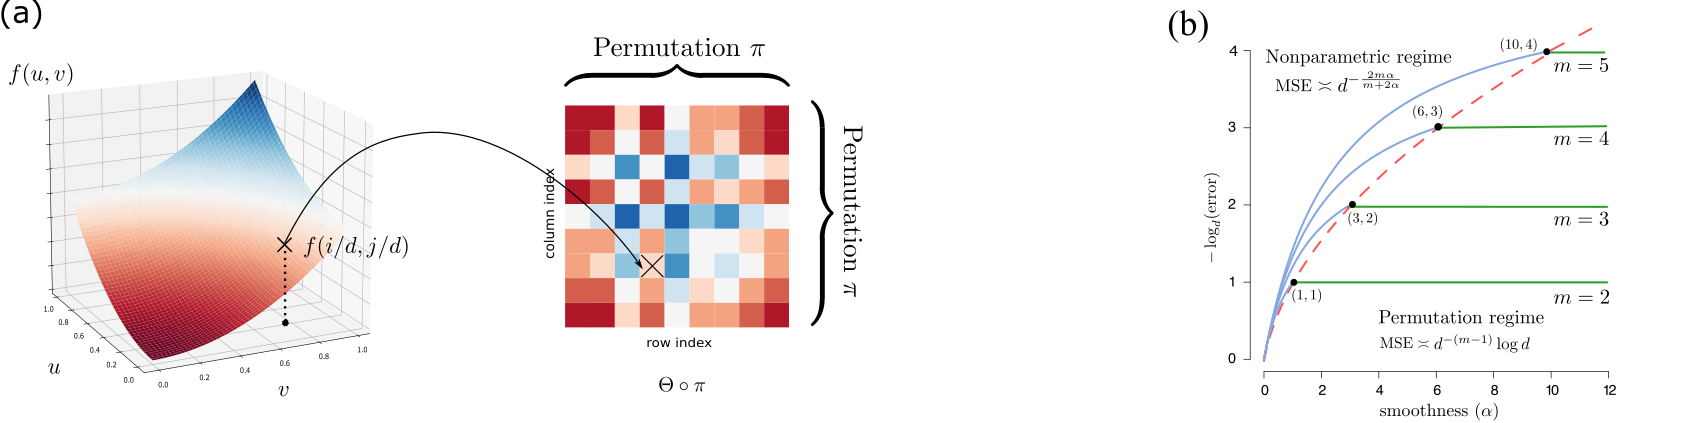
\includegraphics[width = .75\textwidth]{figure/semantic_new.pdf}
    \caption{\small(a): Illustration of order-$m$ $d$-dimensional permuted smooth tensor models with $m=2$. (b): Phase transition of mean squared error (MSE) (on -$\log d$ scale) as a function of smoothness
$\alpha$ and tensor order $m$. Bold dots correspond to the critical smoothness level above which higher
smoothness exhibits no further benefits to tensor estimation; See Theorems~\ref{thm:LSE}-\ref{thm:BC} in the full paper.} \label{fig:rate}
   \vspace{-.2cm}
\end{figure}

The estimation problem of~\eqref{eq:rep} falls into the general category of structured learning with \emph{latent permutation}, which has recently observed a surge of interest. Models involving latent permutations include graphon~\cite{gao2015rate,klopp2017oracle}, stochastic transitivity models~\cite{shah2019low}, and crowd labeling~\cite{li2019nearest}. Most of these methods are developed for matrices. The tensor counterparts are far less well understood. 
%We propose two estimating algorithms with accuracy guarantees: the least square estimation and Borda count estimation. 
In the main paper, we provide statistical and computational estimation accuracy for the permuted smooth tensor model~\eqref{eq:rep}.  Our major contributions are summarized below.

\begin{table*}[http]
    \centering
    \scalebox{0.85}{
    \begin{tabular}{c|cccc}
    & Pananjady et al~\cite{pananjady2020isotonic}&  Balasubramanian~\cite{balasubramanian2021nonparametric}&  Li et al~\cite{li2019nearest}&\textbf{Ours$^*$}\\
    \hline
       Model structure& monotonic & Lipschitz & Lipschitz &  $\alpha$-smoothness  \\
     Minimax lower bound& $\surd$  & $\times$ & $\times$ & $\surd$ \\
 Error rate for order-$m$ tensor$^*$ & \multirow{2}{*}{$d^{-1}$} & $d^{-{2m/(m+2)}}$ & $d^{-\lfloor m/3\rfloor }$ & $d^{-(m-1)}$ \\
       (e.g., when $m=3$) & & ($d^{-6/5}$) & $(d^{-1})$ & $(d^{-2})$ \\

     Polynomial algorithm& $\surd$ &$\times$ & $\surd$ & $\surd$\\
        \hline
    \end{tabular}}
    \caption{\small Comparison of our results with previous works. $^*$We  list here only the result for infinitely smooth order-3 tensors. Our results allow general tensors of arbitrary order $m$ and smoothness $\alpha$.}\label{tab:comp}
\end{table*}
\vspace{-.1cm}
\begin{itemize}[wide,labelwidth=0pt, labelindent=0pt,itemsep=.4ex,topsep=-2pt]
\item We develop a general permuted $\alpha$-smooth tensor model, where $\alpha\geq 0$ is some natural measure of functional smoothness (formal definition in the full paper). In contrast to earlier work~\cite{balasubramanian2021nonparametric,li2019nearest}, we establish the statistically optimal rate and fully characterize its dependence on tensor order, dimension, and smoothness index. Table~\ref{tab:comp} summarizes our improvement over previous works on tensor learning with latent permutations.  We establish the upper bound of the least-square estimate with high probability and show that this upper bound matches with minimax lower bound implying its optimality. 
\vspace{-.2cm}
\item We discover a phase transition phenomenon with respect to the smoothness threshold needed for optimal recovery in model~\eqref{eq:rep}. 
Figure~\ref{fig:rate}(b) plots the dependence of estimation error in terms of smoothness level $\alpha$ for tensors of order $m$. We find that the estimation accuracy improves with smoothness in the regime $\alpha \leq m(m-1)/2$, but then it becomes a constant of $\alpha$ in the regime $ \alpha > m(m-1)/2$. The phenomenon is distinctive from matrix problems~\citep{klopp2017oracle} and classical \emph{non-permuted} smooth function estimation, thereby highlighting the fundamental challenges in our new setting. 
\vspace{-.2cm}
\item We propose two estimation algorithms with accuracy guarantees: the least-squares estimation and Borda count estimation. The least-squares estimation is minimax optimal but computationally hard. The Borda count algorithm is polynomial-solvable, and we show it provably achieves the same optimal rate under extra monotonicity assumptions. Application to Chicago crime analysis is presented to showcase the usefulness of our method. 
\end{itemize}
We believe our results will be of interest to a very broad readership – from those interested in foundations of tensor methods to those in tensor data applications. Our method will help the practitioners efficiently analyze tensor datasets in various areas. Toward this end, the software package and all data used have been publicly released at CRAN.

{\small
\bibliographystyle{plain}\vspace{-.1cm}
\bibliography{tensor_wang}
}



\end{document}
